\section{Introduction}
\label{sec:intro}

Granular computing (GrC) has spent four decades building a principled
toolkit for decision-making under incomplete information.  The conceptual
roots lie in Zadeh's information granularity~\cite{Zadeh1979granularity},
Lin's neighbourhood systems~\cite{Lin1998neighborhood}, and Pedrycz's
programmatic formulation of granular
computing~\cite{Pedrycz2001GrC}.  Starting from
Pawlak's rough sets~\cite{Pawlak1982}, the field has produced a rich theory
of granules (equivalence classes, neighbourhood balls, covering sets),
approximation operators (lower, upper, boundary), and knowledge reduction
(attribute reduct, discernibility).  Neighbourhood rough sets
(NRS)~\cite{Hu2008NRS} extended this framework to continuous data;
granular ball NRS (GBNRS)~\cite{Xia2020GBNRS} further replaced the
fixed-radius ball with a purity-controlled adaptive granule, accumulating
259 citations since 2020 (retrieved September 2025).

The past decade has seen a wave of papers importing frameworks from modern
mathematics and machine learning into this core pipeline.  Persistent
homology offers a multi-scale topological summary of a point cloud.
Fuzzy topology and Alexandrov preorders generalise the equivalence
relation.  Conformal prediction and weak supervision address label
uncertainty.  These are powerful tools; the GrC community's interest in
them is legitimate.

\paragraph{The thesis of this survey.}
Our central finding, supported by a systematic literature review and by
original negative-result experiments, is the following.

\begin{quote}
When a modern mathematical or ML framework is imported into GrC's core
pipeline (neighbourhood granule $\to$ approximation $\to$ reduct), the
resulting quantity tends to either (A) reduce to an already-known
granular quantity, (B) be dominated by geometry of the feature distribution
that is orthogonal to the decision problem, or (C) succeed only where the
evaluation
is aligned with its own objective---whether algebraically, or through a free
parameter of the metric.
\end{quote}

We call these \emph{Pattern A}, \emph{Pattern B}, and \emph{Pattern C}.
Figure~\ref{fig:patterns} locates each pattern in the GrC pipeline and
gives a concrete instantiation; Sections~\ref{sec:patA}--\ref{sec:patC}
provide experimental verification of each.

\begin{figure*}[pos=!htbp]
\centering
\begin{tikzpicture}[
  %% style definitions
  stage/.style  = {draw, rounded corners=5pt, fill=gray!9,
                   minimum width=2.6cm, minimum height=1.1cm,
                   align=center, font=\small},
  import/.style = {draw, rounded corners=5pt, fill=blue!9,
                   minimum width=2.6cm, minimum height=1.1cm,
                   align=center, font=\small},
  patbox/.style = {draw, rounded corners=4pt,
                   minimum width=3.0cm, minimum height=1.55cm,
                   align=center, font=\small},
  patA/.style   = {patbox, fill=blue!11,   draw=blue!55!black},
  patB/.style   = {patbox, fill=orange!16, draw=orange!65!black},
  patC/.style   = {patbox, fill=green!13,  draw=green!55!black},
  arr/.style    = {-{Stealth[length=5pt]}, thick},
  darr/.style   = {-{Stealth[length=5pt]}, thick, dashed},
  lbl/.style    = {font=\scriptsize, midway, above},
]

%% ── Pipeline (top row) ───────────────────────────────────────────────────────
\node[import] (fw)     at (0,0)
  {\textbf{Modern}\\[-2pt]\textbf{framework}\\[1pt]
   \scriptsize TDA, fuzzy topology,\\[-2pt]conformal, weak sup.};

\node[stage, right=1.1cm of fw]   (gran)
  {\textbf{Granule}\\[-2pt]\textbf{geometry}\\[1pt]
   \scriptsize $\delta$-ball, GB, covering};

\node[stage, right=1.1cm of gran] (approx)
  {\textbf{Approx.\ /}\\[-2pt]\textbf{Reduct}\\[1pt]
   \scriptsize $\underline{\mathrm{apr}}$, $\overline{\mathrm{apr}}$, $\mathrm{POS}$, $\gamma$};

\node[stage, right=1.1cm of approx] (eval)
  {\textbf{Evaluation}\\[-2pt]\textbf{metric}\\[1pt]
   \scriptsize accuracy, persistence,\\[-2pt]structure scores};

%% ── Pipeline arrows ──────────────────────────────────────────────────────────
\draw[arr] (fw)     -- node[lbl]{import} (gran);
\draw[arr] (gran)   --                   (approx);
\draw[arr] (approx) --                   (eval);

%% ── Pattern boxes (bottom row) ───────────────────────────────────────────────
\node[patB, below=1.7cm of gran]
  (pB) {\textbf{Pattern B}\\[2pt]
        Label-orthogonal geometry\\dominates the signal\\[3pt]
        \textit{\scriptsize PAI bounded by range$(a_j)$;}\\[-2pt]
        \textit{\scriptsize driven by distribution shape}};

\node[patA, below=1.7cm of approx]
  (pA) {\textbf{Pattern A}\\[2pt]
        New quantity reduces to\\a known granular one\\[3pt]
        \textit{\scriptsize Supervised persistence $\to$ DEP}};

\node[patC, below=1.7cm of eval]
  (pC) {\textbf{Pattern C}\\[2pt]
        Method wins only where\\evaluation aligns with it\\[3pt]
        \textit{\scriptsize PAI wins on Wasserstein;}\\[-2pt]
        \textit{\scriptsize knn-overlap flips with $K$}};

%% ── Downward dashed arrows ────────────────────────────────────────────────────
\draw[darr, orange!65!black] (gran.south)   -- (pB.north);
\draw[darr, blue!55!black]   (approx.south) -- (pA.north);
\draw[darr, green!55!black]  (eval.south)   -- (pC.north);

%% ── Background shading for GrC pipeline ─────────────────────────────────────
\begin{scope}[on background layer]
  \node[fill=gray!5, rounded corners=6pt,
        fit=(gran)(approx)(eval),
        inner sep=6pt, label={[font=\scriptsize\itshape]above:GrC core pipeline}] {};
\end{scope}

\end{tikzpicture}
\caption{Three structural failure patterns arising when a modern mathematical
or ML framework is imported into GrC's core pipeline.
\textbf{Pattern~A}: the new quantity reduces algebraically to a known granular
measure (\S\ref{sec:patA}).
\textbf{Pattern~B}: the importance signal is dominated by label-orthogonal
properties of the feature's distribution---measurement scale being the
special case a stability bound captures (\S\ref{sec:patB}).
\textbf{Pattern~C}: the method wins only where evaluation aligns with its own
objective---algebraically, or via a metric parameter the analyst chooses---and
not on criteria that are robust to that choice (\S\ref{sec:patC}).
Each pattern is diagnosable before implementation (Section~\ref{sec:checklist}).}
\label{fig:patterns}
\end{figure*}

This is not a pessimistic thesis.  Patterns~A--C are diagnostic, not
prohibitive.  They can be checked before implementation
(Section~\ref{sec:checklist}), saving months of wasted work.  And the
nine open problems in Section~\ref{sec:open} are open precisely
because they cannot be solved by a naive import of an existing framework.

\paragraph{Positioning.}
Most surveys in the GrC/rough-set space are taxonomic: they organise
papers by method type and report improvements in mean accuracy.
Yuan et al.~\cite{Yuan2021survey} survey fuzzy rough set attribute reduction
(126 citations); Kuzudisli et al.~\cite{Kuzudisli2023review} survey
grouping-based feature selection (69 citations); Santos et
al.~\cite{Santos2022overlap} survey class overlap complexity (93 citations);
Liu et al.~\cite{Liu2026survey} survey rough feature
selection algorithms across accelerated, incremental, weakly-supervised, and
multi-granularity variants---the broadest scope among these four surveys,
covering several directions that overlap with our Axes~1 and~3.
Liu et al.\ catalogue methods; we diagnose \emph{failure modes} when
external frameworks enter the pipeline, and back the diagnosis with
negative-result experiments that their survey does not attempt.
These are valuable contributions.
Table~\ref{tab:survey_compare} summarises the key differences.

\begin{table}[pos=!htbp]
\caption{Comparison with prior surveys in the GrC / rough-set feature-selection
area.  ``Expt.'' = original experiments; ``Fail.\ diag.'' = failure-pattern
diagnosis; ``Data rel.'' = raw data released.}
\label{tab:survey_compare}
\centering\small
\setlength\tabcolsep{3pt}
\begin{tabular}{p{3.2cm}cccccc}
\toprule
Survey & Scope & Period & \#Papers & Expt. & Fail.\ diag. & Data rel. \\
\midrule
Yuan et al.~\cite{Yuan2021survey}
  & Fuzzy RS reduction & 2000--2020 & 96 & Yes & No & No \\
Kuzudisli et al.~\cite{Kuzudisli2023review}
  & Grouping-based FS & 2010--2022 & 82 & No & No & No \\
Santos et al.~\cite{Santos2022overlap}
  & Class overlap & 2000--2021 & 120 & No & No & No \\
Liu et al.~\cite{Liu2026survey}
  & Rough FS algorithms & 2005--2025 & 150+ & No & No & No \\
\textbf{This survey}
  & GrC + modern math. & 2000--2025 & 52 & Yes & Yes & Yes \\
\bottomrule
\end{tabular}
\end{table}

The closest precursor to our own work is Yuan et al.~\cite{Yuan2021survey},
published in Applied Soft Computing, which surveys fuzzy
rough set attribute reduction methods via comparative experiments on 12 UCI
datasets.  That paper's scope and ours are complementary rather than
overlapping.  Yuan et al.\ cover fuzzy rough set methods---a specific
formal variant of the rough set framework---and evaluate them on mean accuracy
benchmarks.  Our survey covers \emph{what happens when modern mathematical
frameworks} (topology, persistent homology, conformal prediction, weak
supervision) are imported into the broader granular computing pipeline; it
does not survey fuzzy rough sets as a family.  Methodologically, we add what
Yuan et al.\ did not: a falsifiable thesis about structural failure modes,
negative-result experimental evidence, and a critique of the benchmark
methodology used across the community (including papers like those surveyed
in Yuan et al.).

Across these surveys, our work stands apart in being diagnostic rather than
cataloguing: we argue that a specific structural dynamic limits the GrC+X
literature, we provide original experimental evidence for it, and we show
with data---not opinion---that the field's dominant evaluation protocol is
often insensitive to the differences it purports to detect.  Concretely,
this survey contributes:

\begin{enumerate}
  \item \textbf{A falsifiable thesis} (Patterns~A--C) about how imported
        frameworks fail, with an explicit refutation condition for each
        (Sections~\ref{sec:failure} and~\ref{sec:open}).
  \item \textbf{A taxonomy of the topological literature} into two
        branches that our corpus shows to be unconnected, with the
        conditions under which bridging them avoids Pattern~A
        (Section~\ref{sec:topology}).
  \item \textbf{A saturation assessment of granule geometry}
        (Table~\ref{tab:granule_tax}): the natural deformations of the
        neighbourhood ball have each been taken (Section~\ref{sec:geometry}).
  \item \textbf{Original negative-result experiments}---$4{,}975$
        importance measurements and $30{,}100$ classification records,
        released per fold---documenting where a designed-to-succeed method
        fails and why, with a bound (Theorem~\ref{thm:pai_bound}) that
        explains the mechanism (Section~\ref{sec:patB}).
  \item \textbf{A data-driven methodology critique} showing that on seven of
        ten standard benchmarks the best reduct is not statistically
        separable from using every feature, and that across 22 papers read at
        full text---13 of them, a majority of our Axis-1 corpus---not one
        reports all four of an all-features baseline, dispersion, a
        significance test and a hyperparameter ablation, with the per-paper
        coding released for audit (Section~\ref{sec:methodology}).
  \item \textbf{A diagnostic checklist and a six-point reporting standard},
        applicable before implementation (Sections~\ref{sec:checklist}
        and~\ref{sec:standard}), together with nine open problems and the
        barrier that keeps each open (Section~\ref{sec:open}).
\end{enumerate}

Two audiences are addressed directly: the granular-computing researcher
weighing whether to import a modern framework, who should read
Sections~\ref{sec:failure} and~\ref{sec:open} first; and the reviewer or
editor asking why so many GrC feature-selection papers report improvements
that do not replicate, for whom Section~\ref{sec:methodology} is the
relevant part.

\paragraph{Scope.}
The four survey axes are not mutually exclusive: GBNRS appears in both
Axis~1 (geometry) and Axis~3 (efficiency), and three-way decision spans
Axis~1 and Axis~4.  Papers spanning multiple axes are catalogued under
their primary contribution.
We cover the period 2000--2025 with emphasis on 2018--2025, focusing on
feature selection and attribute reduction.  Three-way decision (3WD) and
multi-criteria decision analysis are included where they interact directly
with granule geometry or constitute an actively growing extension of the
core pipeline (Sections~\ref{sec:geo_emerging} and~\ref{sec:trends});
they are not surveyed as standalone paradigms.  We include 52 papers that
passed our inclusion criteria (Appendix~\ref{app:search}); a further 11
background and foundational references are cited as needed.

\paragraph{Organisation.}
Figure~\ref{fig:activity} illustrates the publication-year distribution of
surveyed papers across the four axes: Axis~1 (Granule Geometry) dominates
recent output, while Axes~3 and~4 remain sparse---a pattern that motivates
both the saturation argument (Section~\ref{sec:saturation}) and the open
problems (Section~\ref{sec:open}).
Section~\ref{sec:background} fixes notation.
Sections~\ref{sec:geometry}--\ref{sec:sufficiency} survey the four axes.
Section~\ref{sec:failure} presents the three failure patterns with
experimental evidence.  Section~\ref{sec:methodology} critiques the
field's evaluation practices.  Section~\ref{sec:trends} analyses three
research trends showing sustained momentum---incremental feature selection,
three-way decision integration, and neural-augmented granular
computing---and identifies the conditions under which each avoids the
failure patterns.  Section~\ref{sec:open} lists nine open problems.
Section~\ref{sec:conclusion} concludes.
Figure~\ref{fig:roadmap} provides a bird's-eye view of the survey
structure and the connections between sections.

\begin{figure*}[pos=!htbp]
\centering
\begin{tikzpicture}[
  sec/.style = {draw, rounded corners=4pt, minimum width=2.5cm,
                minimum height=0.85cm, align=center, font=\small,
                fill=gray!8},
  axis/.style = {sec, fill=blue!9, draw=blue!50!black},
  diag/.style = {sec, fill=orange!12, draw=orange!55!black},
  synth/.style = {sec, fill=green!10, draw=green!50!black},
  arr/.style = {-{Stealth[length=4pt]}, thick, gray!60},
  feed/.style = {-{Stealth[length=3.5pt]}, thick, dashed, red!50!black},
]

%% Row 1: Introduction + Background
\node[sec] (s1) at (0, 0) {\S1 Intro\\+ Thesis};
\node[sec] (s2) at (3.2, 0) {\S2 Background\\+ Notation};

%% Row 2: Four Axes
\node[axis] (s3) at (-1.6, -1.5) {\S3 Geometry};
\node[axis] (s4) at (1.6, -1.5) {\S4 Topology};
\node[axis] (s5) at (4.8, -1.5) {\S5 Efficiency};
\node[axis] (s6) at (8.0, -1.5) {\S6 Sufficiency};

%% Row 3: Diagnostic + Trends
\node[diag] (s7) at (1.6, -3.2) {\S7 Failure\\Patterns A/B/C};
\node[diag] (s8) at (4.8, -3.2) {\S8 Methodology\\Critique};
\node[synth] (s9) at (8.0, -3.2) {\S9 Trends};

%% Row 4: Open Problems + Conclusion
\node[synth] (s10) at (3.2, -4.7) {\S10 Open\\Problems (8)};
\node[sec]  (s11) at (6.4, -4.7) {\S11 Conclusion};

%% Forward arrows
\draw[arr] (s1) -- (s2);
\draw[arr] (s2) -- (s3); \draw[arr] (s2) -- (s4);
\draw[arr] (s2) -- (s5); \draw[arr] (s2) -- (s6);
\draw[arr] (s3) -- (s7); \draw[arr] (s4) -- (s7);
\draw[arr] (s5) -- (s7); \draw[arr] (s6) -- (s7);
\draw[arr] (s7) -- (s8);
\draw[arr] (s6) -- (s9);
\draw[arr] (s7) -- (s9);
\draw[arr] (s8) -- (s10);
\draw[arr] (s9) -- (s10);
\draw[arr] (s10) -- (s11);

%% Feedback arrows (failure patterns feed back to axes)
\draw[feed] (s7.north) to[bend left=18] node[font=\scriptsize, above, sloped]
  {A/B/C diagnostic} (s3.south east);

\end{tikzpicture}
\caption{Bird's-eye view of the survey structure.  Blue boxes: the four
survey axes (Sections~\ref{sec:geometry}--\ref{sec:sufficiency}).  Orange
boxes: the diagnostic programme (failure patterns and methodology critique).
Green boxes: synthesis (trends and open problems).  Dashed arrow: the A/B/C
failure-pattern diagnostic feeds back into the assessment of each axis.}
\label{fig:roadmap}
\end{figure*}

\begin{figure*}[pos=!htbp]
\centering
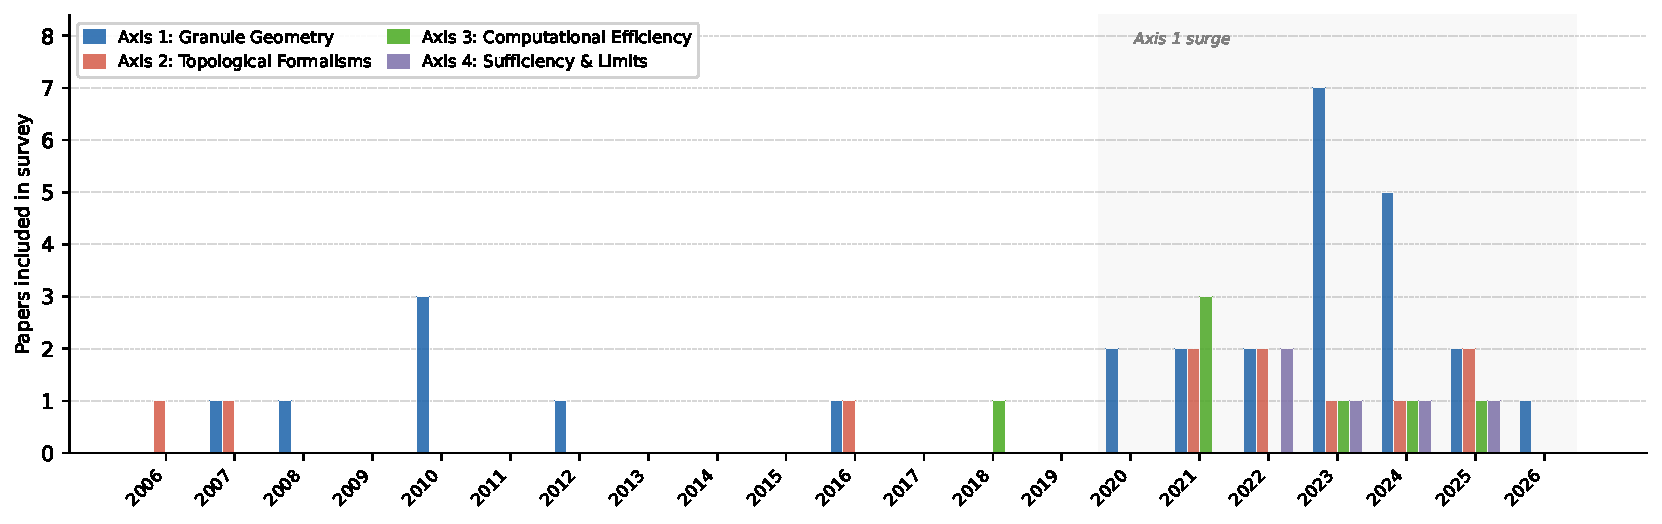
\includegraphics[width=\textwidth]{figures/activity_by_axis.pdf}
\caption{Publication-year distribution of the 52 included papers across the
four research axes (2006--2026).  Background and foundational references
(11 papers: TDA stability theorems, learning-theory bounds, survey references)
are not plotted.  Axis~1 (Granule Geometry) dominates output since 2020,
supporting the saturation argument of Section~\ref{sec:saturation}.
The shaded region marks the 2020--2026 surge period.}
\label{fig:activity}
\end{figure*}
